\chapter{\chapTwo}
\label{cha:chapter2} % Label for hyperlink

% Start font-size
\begingroup
\fontsize{12pt}{14pt}\selectfont

\section{OpenCV}
\label{sec:ocv} % Label for hyperlink
OpenCV steht für \enquote{Open Source Computer Vision Library} und ist eine der umfangreichsten Bibliotheken für die Echtzeit-Verarbeitung visueller Daten.
Das \enquote{Open} im Namen weist darauf hin, dass es sich um ein Open-Source-Projekt handelt.
Der Quelltext ist also öffentlich zugänglich und darf unter Einhaltung der Lizenzbedingungen verändert und kostenfrei verwendet werden.
OpenCV stellt mehrere sogenannte \textit{Dictionaries} bereit, die im Folgenden als \enquote{Bibliotheken} bezeichnet werden.

Die Bibliothek OpenCV wurde in C\texttt{++} implementiert, um eine hohe Rechenleistung, Plattformunabhängigkeit und eine modulare Struktur zu gewährleisten.
Auf Basis des C\texttt{++}-Kerns sind später Schnittstellen für Python, Java und andere Sprachen entstanden, die die Nutzung der Bibliothek erleichtern \cite{ocv:org}\footnote{\url{opencv.org/about}}.

\subsection{Einsatzbereiche}
OpenCV findet Anwendung in vielen Bereichen der Bildverarbeitung.
Die Bibliothek eignet sich insbesondere für Aufgaben, die eine effiziente Verarbeitung von Bildern und Videos in Echtzeit erfordern.
Einige typische Beispiele sind in der folgenden Liste dargestellt \cite{Wiki:ocv}.

\begin{minipage}{0.55\textwidth}
    \begin{enumerate}
        \item Automatisierte Gesichtserkennung
        \item Gestenerkennung
        \item Bewegungsanalyse
        \item Objektidentifizierung
    \end{enumerate}
\end{minipage}
\hfill
\begin{minipage}{0.4\textwidth}
    \begin{figure}[H]
        \centering
            
\includegraphics[width=0.5\textwidth]{ocv_logo.pdf}
        \caption{Logo von OpenCV \cite{ocv:org}.}
            \label{pic:ocv_logo}
    \end{figure}
\end{minipage}

Abgesehen von diesen klassischen Anwendungsfeldern wird OpenCV auch zunehmend in Forschungsprojekten genutzt, beispielsweise zur Gesten- oder Marker-basierten Steuerung von Robotiksystemen, wie sie im Rahmen dieser Arbeit zum Einsatz kommt \cite{sse:foodDel}.

\subsection{Module}
OpenCV ist modular aufgebaut.
Die Bibliothek besteht aus mehreren unabhängigen, aber miteinander kompatiblen Modulen, die jeweils bestimmte Aufgabenbereiche der Bildverarbeitung abdecken.
Durch diesen Aufbau können nur jene Module eingebunden werden, die für ein Projekt tatsächlich benötigt werden, was den Speicherbedarf reduziert und die Effizienz erhöht.
In \aTeLi{tab:ocvModules} sind drei zentrale Module von OpenCV aufgeführt:

\begin{table}[H]
    \begin{tabularx}{\textwidth}{l X}

        \toprule
        \multicolumn{1}{c}{\textbf{Modul}} & \multicolumn{1}{c}{\textbf{Beschreibung}} \\
        \midrule

        \texttt{core} & Das core-Modul ist das Grundgerüst von OpenCV. Es stellt grundlegende Datenstrukturen, Matrizenoperationen und mathematische Funktionen bereit, die von anderen Modulen verwendet werden.\\
        \addlinespace[3pt]

        \texttt{imgproc} & Das imgproc-Modul bietet eine umfassende Reihe von Bildverarbeitungsfunktionen.\\
        \addlinespace[3pt]

        \texttt{aruco} & Das aruco-Modul ermöglicht die Erkennung und Verarbeitung von \hTeLi{sec:aruco}{ArUco-Markern}. Es kann die Position und Orientierung der Marker berechnen und ist das wichtigste Modul dieser Arbeit.\\
        \bottomrule
    \end{tabularx}
    \caption{Wichtige Module der OpenCV-Bibliothek \cite{ocv:docs}.}
        \label{tab:ocvModules}
\end{table}

Die modulare Struktur erlaubt es, OpenCV sowohl in ressourcenbeschränkten Systemen, wie zum Beispiel bei Drohnen oder eingebetteten Geräten, als auch in komplexen Computer-Vision-Projekten effizient einzusetzen.

\section{ArUco-Marker}
\label{sec:aruco}
Ein ArUco-Marker (wie in \aTeLi{pic:marker0} dargestellt) ist ein quadratischer Referenzmarker, der zur Positions- und Orientierungserkennung in Bildern bzw. Kamerasystemen zum Einsatz kommt.
Referenzmarker (auch Passermarken) werden ursprünglich in automatisierten Fertigungsverfahren von elektronischen Bauelementen wie beispielsweise Hauptplatinen verwendet.
Sie dienen als optische Referenzpunkte für die Maschinen, die am Fertigungsprozess beteiligt sind.
Dadurch erhöhen sie die Präzision und reduzieren Kurzschlüsse \cite{Wiki:Passermarke}.

Es gibt Referenzmarker in verschiedenen Grössen, Farbschemen und Formen, abhängig von ihrem Einsatzgebiet.
Für diese Arbeit werden aus folgenden Gründen quadratische benutzt:

\begin{itemize}
    \item Die Erkennung der Marker erfolgt schnell und effizient, was bei Echtzeitsteuerung vorteilhaft ist.
    \item Quadratische Marker werden häufig gebraucht und sind daher ausführlicher dokumentiert als andere.
    \item Sie sind relativ einfach einzusetzen.
\end{itemize}

ArUco-basierte Marker zählen zu den verlässlichsten, vor allem seit \hTeLi{sec:ocv}{OpenCV} ein Submodul zur Implementierung dieser Marker hinzugefügt hat \cite{IJ:fiducial}.

\begin{figure}[H]
    \centering
        
\includegraphics[width=0.3\textwidth]{aruco.pdf}
    \caption{ArUco-Marker mit ID 0. Generiert von \cite{chev:arucogen}}.
        \label{pic:marker0}
\end{figure}

\subsection{Funktionsweise}
\label{sub:fw}
Das Schwarzweiss-Schema von ArUco-Markern erinnert an das eines QR-Codes.
Während beide einem ähnlichen Zweck dienen, nämlich der visuellen Identifizierung von Objekten, ist ihr geometrischer Aufbau grundverschieden \cite{ten:qrcode}.
Die Fabrikation von QR-Codes beruht auf drei Hauptbestandteilen:

\begin{enumerate}
    \item Menge der codierten Information.
    \item Modus, in dem die Daten codiert wurden.
    \item Stärke der Fehlerkorrekturfunktion.
\end{enumerate}

Der entscheidende Unterschied zwischen dieser Funktionsweise und der von ArUco-Markern ist der Informationgehalt.
Bei ArUco-Markern existiert dieser nicht.
Sie sind nicht eine binäre Übersetzung einer vordefinierten Eingabe, sondern sind in nummerierten Bibliotheken angelegt und besitzen keine versteckte Botschaft.
Es gibt keinen Algorithmus, der Klartext in einen ArUco-Marker übersetzt.
Dieses Konzept hat seine Vor- und Nachteile.
Einerseits erhöht es die Geschwindigkeit der Identifizierung, andererseits limitiert es die Gesamtmenge aller Marker.
Diese Bedingungen sind jedoch ideal für dieses Projekt, da nur wenige verschiedene Marker benötigt werden und Effizienz gefragt ist.

Um einen gesuchten Marker in den Bibliotheken zu finden, braucht man den Namen der Bibliothek und die ID des Markers.
Der Name der Bibliothek legt die Grösse der Matrix und somit Komplexität des Markers fest sowie die Anzahl möglicher Marker.

In der Tabelle \aTeLi{tab:arucoDicts} sind drei Bibliotheken und deren Eigenschaften dargestellt.
Es ist zu beachten, dass alle Marker der Bibliothek \bodyCode{DICT\_4X4\_50} auch in \bodyCode{DICT\_4X4\_100} vorhanden sind, da die grössere Bibliothek alle IDs der kleineren umfasst.
Für dieses Projekt wird die Bibliothek \bodyCode{DICT\_4X4\_50} verwendet, weil es die geometrisch unkomplizierteste Bibliothek ist, die OpenCV unterstützt.
Das ist insofern wichtig, weil die Marker letztendlich unter Winkeln bis zu 45° erkennbar sein sollen.
Da weitaus weniger als fünfzig Marker benötigt werden, reicht die \bodyCode{\_50} Bibliothek aus.

\begin{table}[H]
    \centering
    \begin{tabular}{lcc}
        \toprule
        \textbf{Bibliothek} & \textbf{Datenbits} & \textbf{Markeranzahl} \\
        \midrule

        \bodyCode{DICT\_4X4\_50} & 16 & 50 \\
        \addlinespace[3pt]

        \bodyCode{DICT\_4X4\_100} & 16 & 100 \\
        \addlinespace[3pt]

        \bodyCode{DICT\_5X5\_50} & 25 & 50 \\
        \bottomrule
    \end{tabular}
    \caption{Eigenschaften ausgewählter ArUco-Dictionaries.}
        \label{tab:arucoDicts}
\end{table}

\section{Mathematische Grundlagen}

In diesem Kapitel werden die für das Verständnis dieser Arbeit benötigten mathematischen Grundlagen erläutert.
Dabei handelt es sich um grundlegende mathematische Konzepte, die für die Auswertung der Bildaten von Nöten sind.

\subsection{NumPy-Arrays und zweidimensionale Listen}
\label{sub:numpy}
NumPy ist eine Python-Bibliothek, die für numerische Berechnungen optimiert ist und in der Regel automatisch mitinstalliert wird, wenn OpenCV installiert wird.
Ein NumPy-Array ist eine Datenstruktur, die numerische Werte in einer festen, mehrdimensionalen Form speichert.
Damit lassen sich Vektor- und Matrixoperationen effizient und direkt ausführen, was insbesondere bei grossen Datensätzen oder komplexen Berechnungen von Vorteil ist.

Im Rahmen dieser Arbeit werden NumPy-Arrays vor allem als Zwischenergebnis bei der Marker-Erkennung durch OpenCV erzeugt.
Da für die weitere Verarbeitung jedoch nur einfache Operationen wie das Durchlaufen und Vergleichen von Koordinaten notwendig sind, werden diese Arrays in zweidimensionale Python-Listen umgewandelt.
Dies vereinfacht den Zugriff auf einzelne Werte und vermeidet die zusätzlichen Strukturen, die NumPy für umfangreiche mathematische Berechnungen bereitstellt.

\subsection{Flächenberechnung mit Gausschen Trapezformel}
\label{sub:gauTrap}

Die Gaussche Trapezformel dient zur Berechnung der Fläche \inlinemath{A} von ebenen, unregelmässigen Polygonen. Sie lautet wie folgt:
\[
2A = \left| \sum_{i=1}^{n} \big((x_i - x_{i+1}) \cdot (y_i + y_{i+1}) \big) \right|
\]
Dabei bezeichnet \inlinemath{n} die Anzahl der Eckpunkte des Polygons, sowie \inlinemath{x_i} und \inlinemath{y_i} die Koordinaten des \inlinemath{i}-ten Punktes im zweidimensionalen Raum.

Wird der Klammerausdruck ausmultipliziert, ergibt sich:
\[
2A = \left| \sum_{i=1}^{n} \big( x_i y_i + x_i y_{i+1} - x_{i+1} y_i - x_{i+1} y_{i+1} \big) \right|
\]
Da gilt, dass sich die Terme \inlinemath{x_i y_i} und \inlinemath{x_{i+1} y_{i+1}} innerhalb der Summe gegenseitig aufheben.
Nach der Kürzung bleibt nur Folgendes übrig:
\[
2A = \left| \sum_{i=1}^{n} \big( x_i y_{i+1} - x_{i+1} y_i \big) \right|
\]
Diese Form entspricht der sogenannten \textit{Shoelace formula} („Schnürsenkel-Formel“), die insbesondere in der Informatik und Bildverarbeitung Anwendung findet.
Sie stellt eine kompakte und praktisch gut anwendbare Variante der Gausschen Trapezformel dar.\footnotemark
\footnotetext{Siehe \hTeLi{tab:tools}{Hilfsmittelverzeichnis}.}
Der Ursprung ihres Namens ist in \aTeLi{pic:polygon} und \aTeLi{pic:shoelace} illustriert.\footnotemark
\footnotetext{Beide Abbildungen inspiriert durch \cite{Wiki:traFormel}.}

\begin{figure}[H]
    \centering
    \begin{subfigure}[t]{0.47\textwidth}
        \centering
        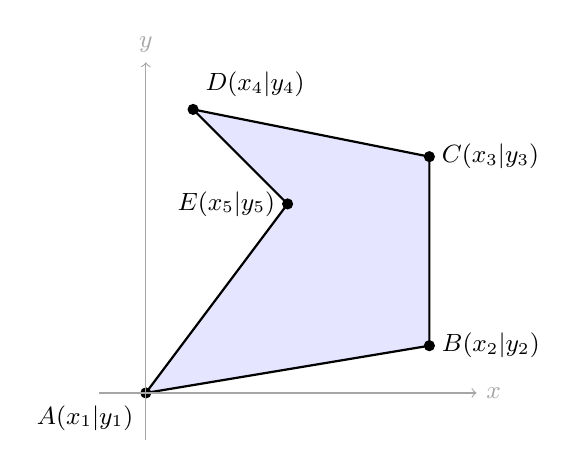
\begin{tikzpicture}[scale=1.2, every node/.style={font=\small}]
            
            % Points
            \coordinate (A) at (0.0,0.0);
            \coordinate (B) at (3.0,0.5);
            \coordinate (C) at (3.0,2.5);
            \coordinate (D) at (0.5,3.0);
            \coordinate (E) at (1.5,2.0);

            % Area
            \fill[blue!10] (A)--(B)--(C)--(D)--(E)--cycle;

            % Sides
            \draw[thick] (A)--(B)--(C)--(D)--(E)--cycle;

            % Point names
            \filldraw[black] (A) circle (1.5pt)
                node[below left=1pt] {$A(x_1|y_1)$};

            \filldraw[black] (B) circle (1.5pt)
                node[right=1pt] {$B(x_2|y_2)$};

            \filldraw[black] (C) circle (1.5pt)
                node[right=1pt] {$C(x_3|y_3)$};

            \filldraw[black] (D) circle (1.5pt)
                node[above right=1pt] {$D(x_4|y_4)$};

            \filldraw[black] (E) circle (1.5pt)
                node[left=1pt] {$E(x_5|y_5)$};

            % Axis
            \draw[->, gray!70] (-0.5,0) -- (3.5,0) node[right] {$x$};
            \draw[->, gray!70] (0,-0.5) -- (0,3.5) node[above] {$y$};
        \end{tikzpicture}
        \caption{Ein Polygon.}
            \label{pic:polygon}
    \end{subfigure}%
    \hfill
    \begin{subfigure}[t]{0.5\textwidth}
        \centering
        \begin{tikzpicture}[node distance=1.5cm, every node/.style={circle, draw, minimum size=8mm, align=center}]
            % Upper circles
            \node (X1) {\inlinemath{x_1}};
            \node (X2) [right of=X1] {\inlinemath{x_2}};
            \node (X3) [right of=X2] {\inlinemath{x_3}};
            \node (X4) [right of=X3] {\inlinemath{x_4}};
            \node (X5) [right of=X4] {\inlinemath{x_5}};
            \node (X6) [right of=X5] {\inlinemath{x_1}};

            % Lower circles
            \node (Y1) [below=2cm of X1] {\inlinemath{y_1}};
            \node (Y2) [right of=Y1] {\inlinemath{y_2}};
            \node (Y3) [right of=Y2] {\inlinemath{y_3}};
            \node (Y4) [right of=Y3] {\inlinemath{y_4}};
            \node (Y5) [right of=Y4] {\inlinemath{y_5}};
            \node (Y6) [right of=Y5] {\inlinemath{y_1}};

            % Point Names
            \node[above=0.3cm of X1, circle=false, draw=none] {\inlinemath{A}};
            \node[above=0.3cm of X2, circle=false, draw=none] {\inlinemath{B}};
            \node[above=0.3cm of X3, circle=false, draw=none] {\inlinemath{C}};
            \node[above=0.3cm of X4, circle=false, draw=none] {\inlinemath{D}};
            \node[above=0.3cm of X5, circle=false, draw=none] {\inlinemath{E}};
            \node[above=0.3cm of X6, circle=false, draw=none] {\inlinemath{A}};

            % Shoelaces
            \draw[->, plusGreen, thick] (X1) -- (Y2);
            \draw[->, plusGreen, thick] (X2) -- (Y3);
            \draw[->, plusGreen, thick] (X3) -- (Y4);
            \draw[->, plusGreen, thick] (X4) -- (Y5);
            \draw[->, plusGreen, thick] (X5) -- (Y6);

            \draw[->, minusRed, thick] (X2) -- (Y1);
            \draw[->, minusRed, thick] (X3) -- (Y2);
            \draw[->, minusRed, thick] (X4) -- (Y3);
            \draw[->, minusRed, thick] (X5) -- (Y4);
            \draw[->, minusRed, thick] (X6) -- (Y5);
        \end{tikzpicture}
        \caption{Schnürsenkel-Muster.}
        \label{pic:shoelace}
    \end{subfigure}
    \caption{Illustrationen zur Shoelace Formula.}
    \label{fig:overall}
\end{figure}

Setzt man die \inlinemath{x}- und \inlinemath{y}-Werte für die einzelnen Punkte ein, so erhält man die doppelte Fläche des Polygons (hier Pentagon).

\begin{minipage}[t]{0.2\textwidth}
    \begin{align*}
        x_n &| y_n \\[3pt]
        A(0.0 &| 0.0) \\
        B(3.0 &| 0.5) \\
        C(3.0 &| 2.5) \\
        D(0.5 &| 3.0) \\
        E(1.5 &| 2.0)
    \end{align*}
\end{minipage}
\vline
\begin{minipage}[t]{0.7\textwidth}
    \begin{align*}
        2A = |&\cp (x_1 \cdot y_2) \cp (x_2 \cdot y_3) \cp (x_3 \cdot y_4) \cp (x_4 \cdot y_5) \cp (x_5 \cdot y_1) \\
        &\cm (x_2 \cdot y_1) \cm (x_3 \cdot y_2) \cm (x_4 \cdot y_3) \cm (x_5 \cdot y_4) \cm (x_1 \cdot y_5)| \\[3pt]
        = |&\cp (0.0 \cdot 0.5) \cp (3.0 \cdot 2.5) \cp (3.0 \cdot 3.0) \cp (0.5 \cdot 2.0) \cp (1.5 \cdot 0.0) \\
        &\cm (3.0 \cdot 0.0) \cm (3.0 \cdot 0.5) \cm (0.5 \cdot 2.5) \cm (1.5 \cdot 3.0) \cm (0.0 \cdot 2.0)| \\[3pt]
        = |&\cp 0.0 \cp 7.5 \cp 9.0 \cp 1.0 \cp 0.0 \cm 0.0 \cm 1.5 \cm 1.25 \cm 4.5 \cm 0.0| \\[3pt]
        = |&\cp 10.25|
    \end{align*}
\end{minipage}

Am Ende muss noch mit \inlinemath{\frac{1}{2}} multipliziert werden, um das korrekte Ergebnis zu erhalten: \inlinemath{A = 5.125}

\subsection{Mittelpunkt eines Vierecks berechnen}
Die Berechnung des Mittelpunktes eines Vierecks ist sehr einfach, weswegen hier nur die Formel angegeben wird:
\[
M_x = \frac{x_1 + x_2 + x_3 + x_4}{4}, \quad M_y = \frac{y_1 + y_2 + y_3 + y_4}{4}
\]
\subsection{Distanzberechnung mittels Vektorsubtraktion}
Jegliche Distanze werden in dieser Arbeit durch die Subtraktion von Vektoren berechnet.
Dazu werden zuerst die Ortsvektoren der Punkte \inlinemath{A(x_1|y_1)} und \inlinemath{B(x_2|y_2)} bestimmt.
\[
\overrightarrow{OA} = \vect{x_1}{y_1}, \quad \overrightarrow{OB} = \vect{x_2}{y_2}
\]
Anschliessend muss der Vektor \inlinemath{\overrightarrow{AB}} berechnet werden.
Das geschieht durch Vektorsubtraktion:
\[
\overrightarrow{AB} = \overrightarrow{OA} - \overrightarrow{OB} = \vect{x_1}{y_1} - \vect{x_2}{y_2} = \vect{x_1-x_2}{y_1-y_2} = \vect{x_3}{y_3}
\]
Zum Schluss muss nur noch der \textit{Satz des Pythagoras} angewendet werden, um die Länge \inlinemath{|\overrightarrow{AB}|} zu berechnen.
\[
|\overrightarrow{AB}| = \sqrt{(x_3)^2 + (y_3)^2}
\]

\section{Crazyflie}
\label{sec:cf}

Als Drohne für diese Arbeit wurde die Crazyflie~2.0 ausgewählt.
Die Eigenschaften, welche \textbf{für} die Wahl dieses Quadrokopters in Forschungsprojekten sprechen, sind im Folgenden aufgelistet:

\begin{itemize}
    \item \textbf{Gewicht:} Die Drohne ist sehr leicht, was vor allem für Einsteiger praktisch ist, da sie weniger anfällig für Beschädigung ist.
    \item \textbf{API:} Bitcraze stellt eine Open-Source-Python-Schnittstelle zur Verfügung, die eine direkte Programmierung der Drohne ermöglicht und damit zentral für diese Arbeit ist (siehe \hTeLi{sub:cflib}{Kapitel~CFLib}).
    \item \textbf{Modularitär:} Es existieren über 15 optionale Erweiterungs-Decks, die den Anwendungsbereich der Crazyflie gezielt erweitern.
\end{itemize}

Im Rahmen dieser Arbeit wird ausschliesslich das in \hTeLi{sub:v2}{Kapitel~\ref{sub:v2}} beschriebene \techWord{Flow-Deck V2} als Erweiterung verwendet.

Inziwschen ist mit \techWord{Crazyflie 2.1\texttt{+}} eine neue Version der erschienen.
Diese wurde mit einer längeren Flugzeit und verbesserten Flugleistung. 

Beide Versionen der Crazyflie sind mit folgenden Funktionen ausgestattet:

\begin{itemize}
    \item Unterstützung der Steuerung über Apple- und Anroid-Smartphones via BLE (Bluetooth Low Energy) sowie über Computer mit angeschlossenem \hTeLi{sec:crpa}{Crazyradio~PA}.
    \item Einem dreiachsigen Gyrosensor.\footnotemark
    \item Einem dreiachsigen Beschleunigungssensor.\footnotemark[\value{footnote}]
    \item Einem dreiachsigen Magnetometer.\footnotemark[\value{footnote}]
    \item Einem Hochpräzision-Drucksensor.
\end{itemize}

\footnotetext{Bestandteil des \techWord{MPU-9250}-Bauteils.}

\begin{figure}[H]
    \centering
    \begin{imgbox}
        \begin{subfigure}[b]{0.3\textwidth}
            \centering
            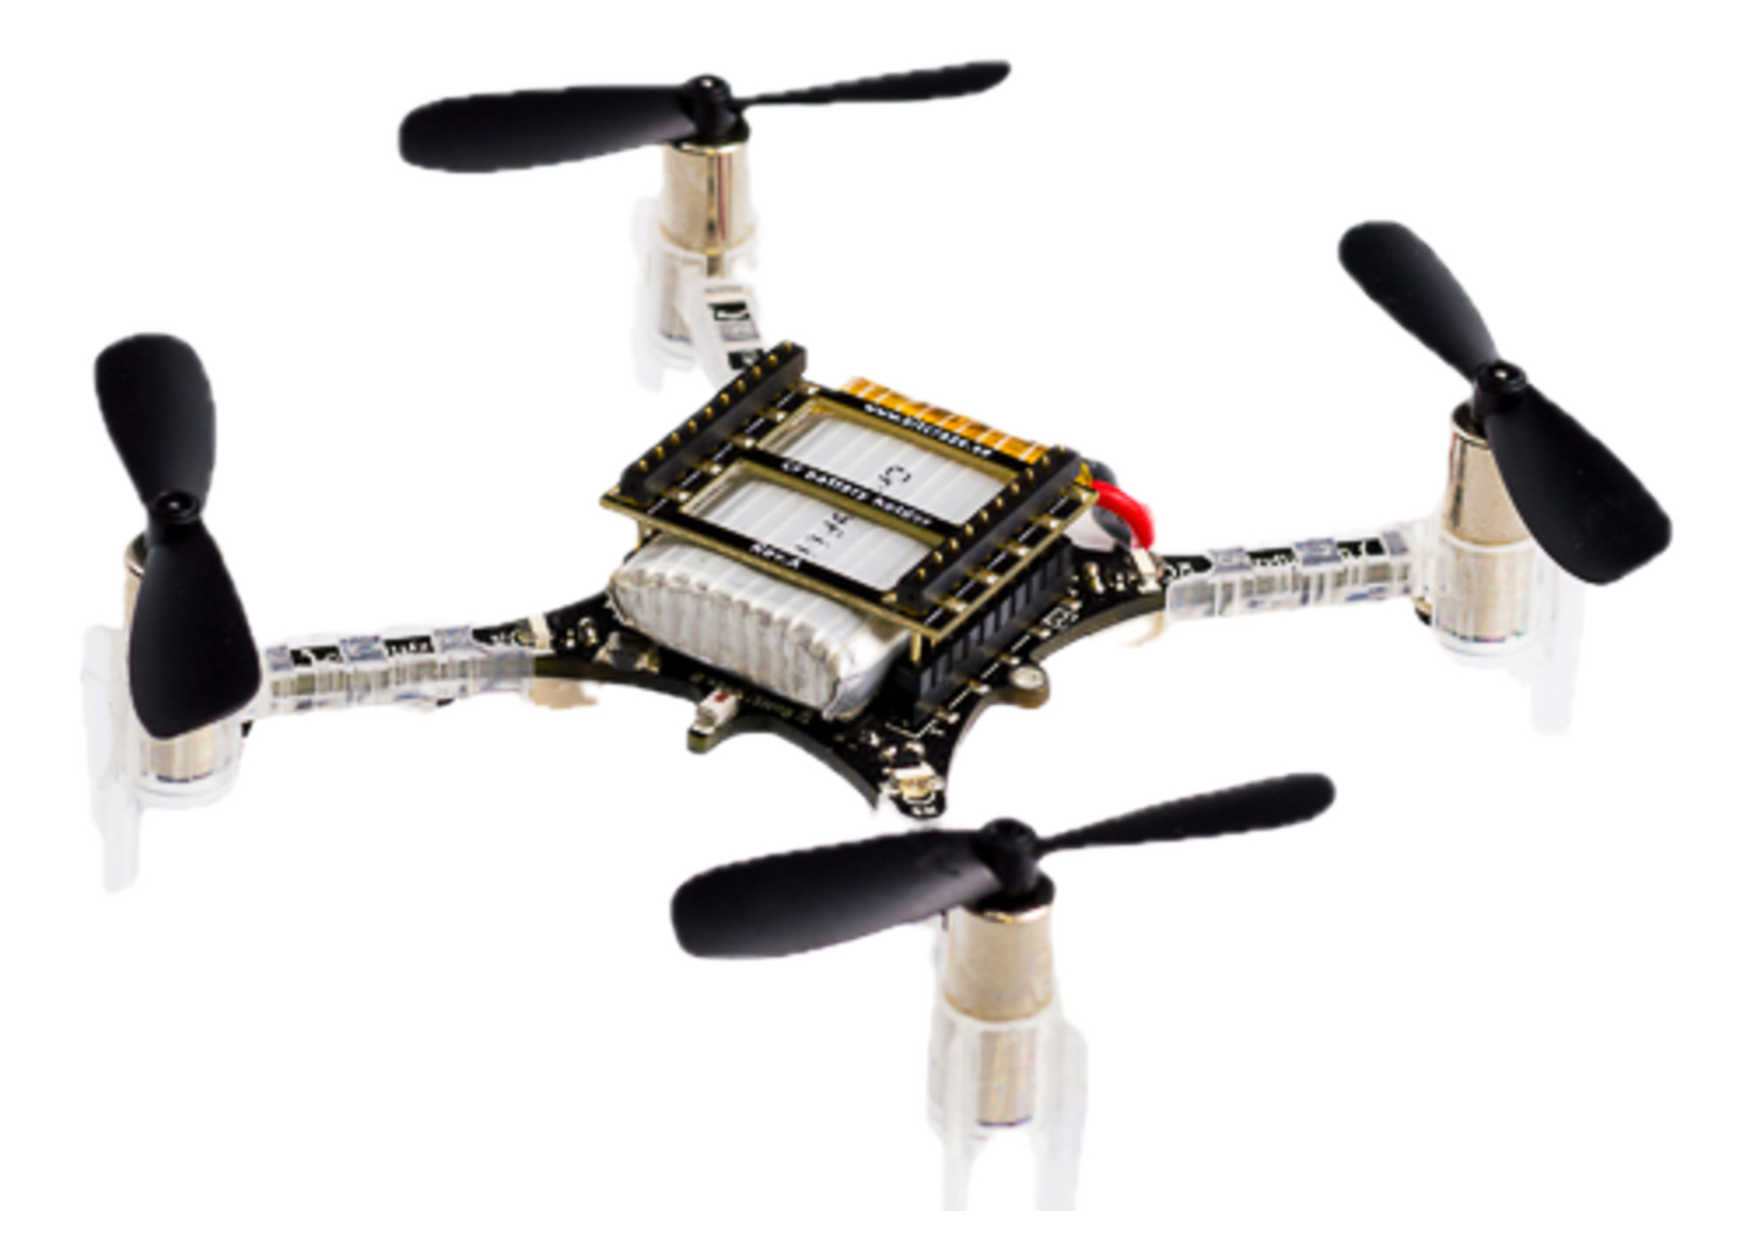
\includegraphics[width=\textwidth]{cf.pdf}
            \caption{Crazyflie \bodyCode{2.0} \cite{bc:cf20}}
            \label{pic:cf20}
        \end{subfigure}
        \hfill
        \begin{subfigure}[b]{0.3\textwidth}
            \centering
            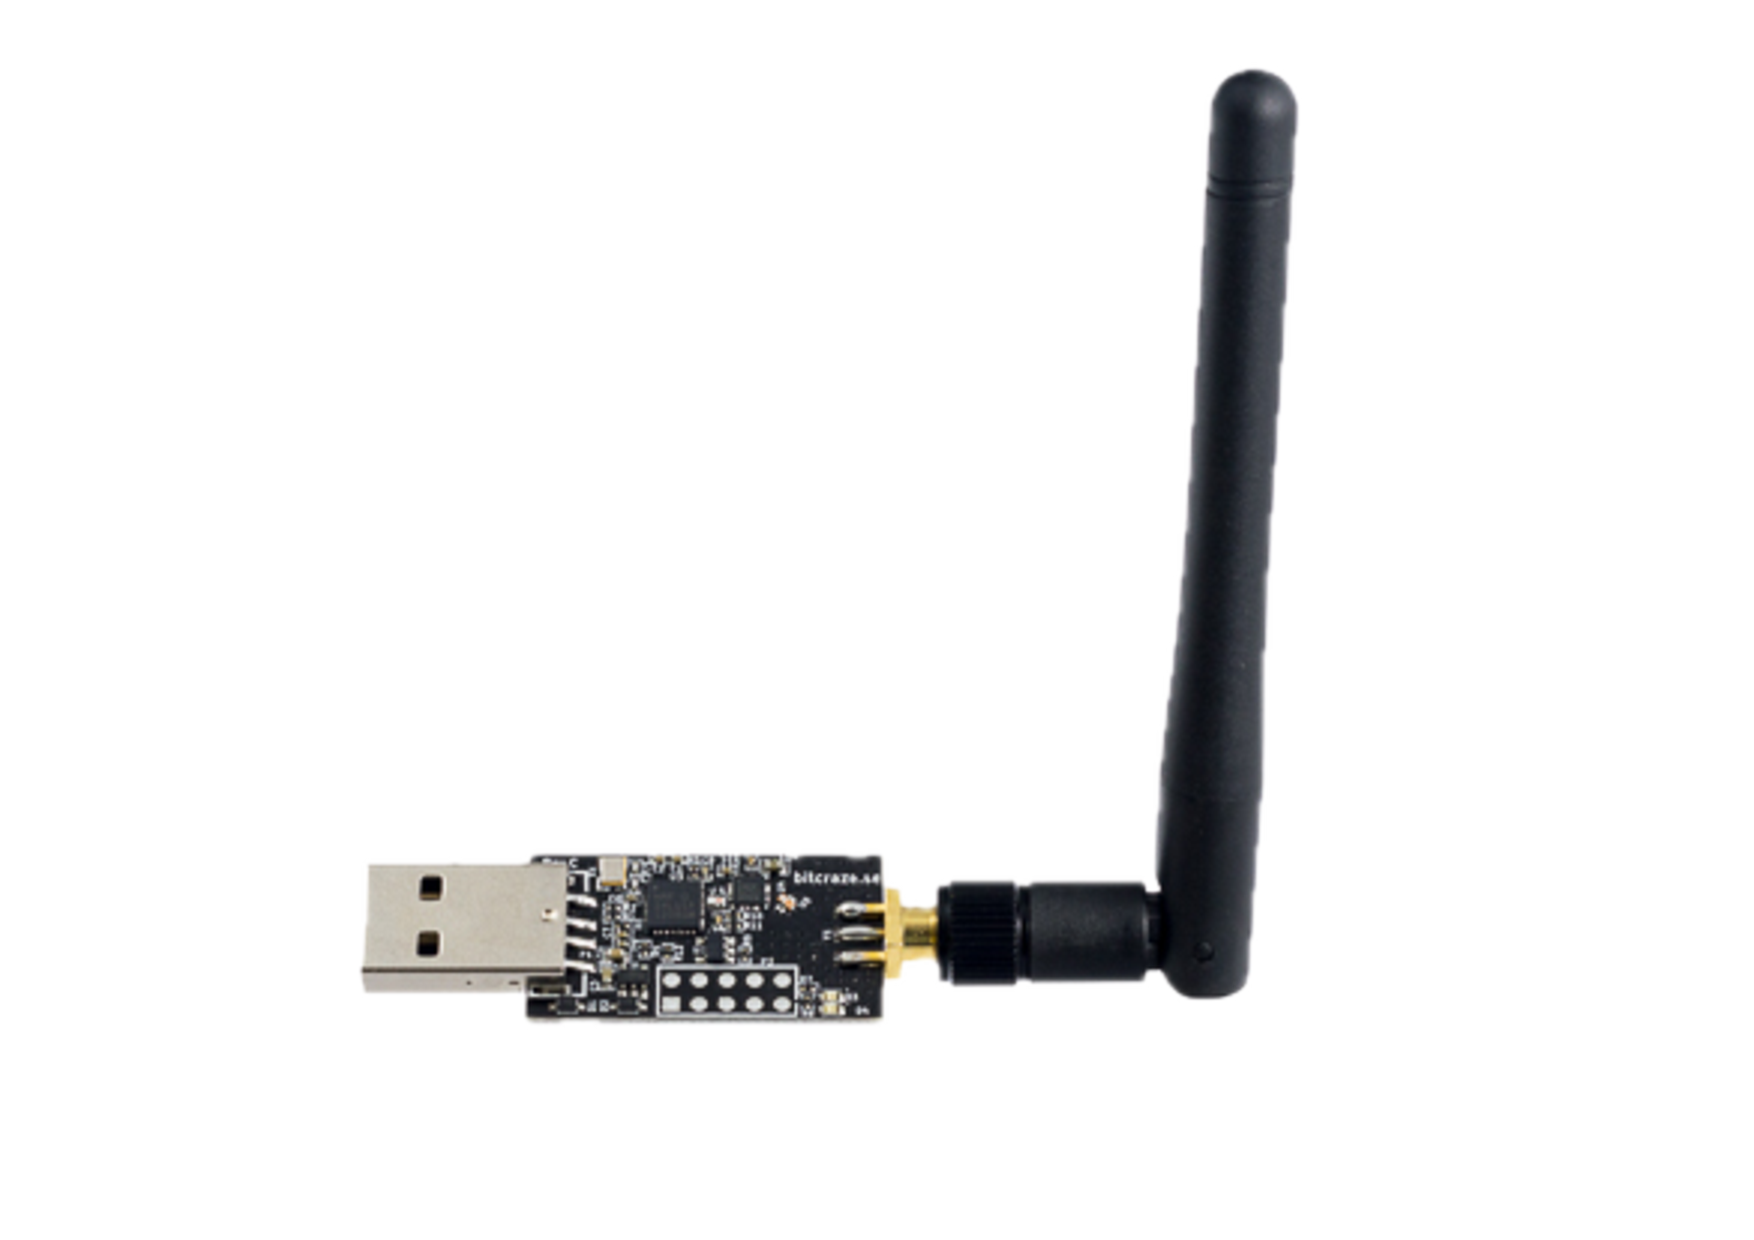
\includegraphics[width=\textwidth]{crpa.pdf}
            \caption{Crazyradio PA \cite{bc:crpa}}
            \label{pic:crpa}
        \end{subfigure}
        \hfill
        \begin{subfigure}[b]{0.3\textwidth}
            \centering
            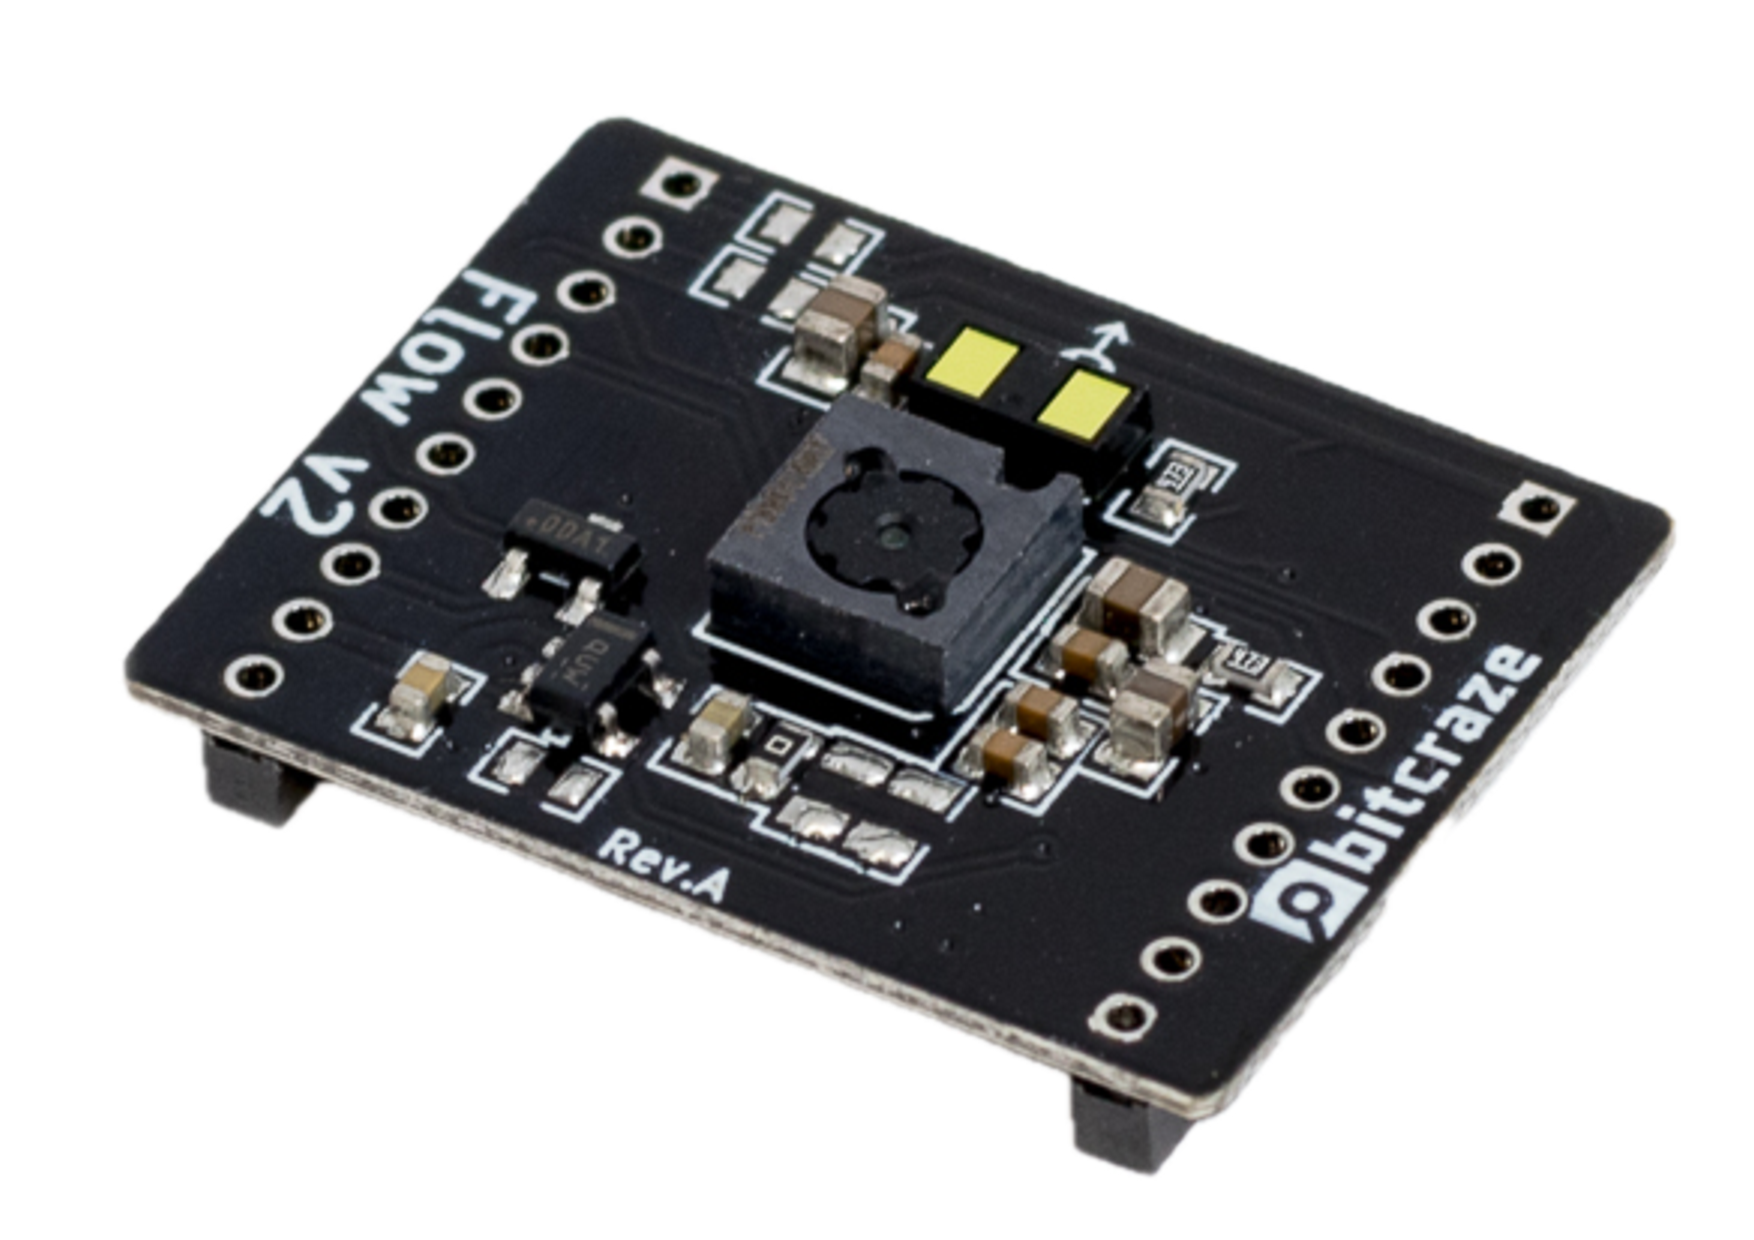
\includegraphics[width=\textwidth]{fdv2.pdf}
            \caption{Flow-Deck V2 \cite{bc:fdv2}}
            \label{pic:fdv2}
        \end{subfigure}
    \end{imgbox}
    \caption{Physische Komponenten}
        \label{fig:drohne_und_radio}
\end{figure}

\subsection{Flow-Deck V2}
\label{sub:v2}

Das Flow-Deck~V2 ist ein Erweiterungsmodul, das an der Unterseite der Drohne befestigt wird.
Es ermöglicht der Crazyflie, ihre absolute Position relativ zur darunterliegenden Oberfläche zu bestimmen.
Das Deck kombiniert einen \techWord{VL53L1x}-ToF-Sensor\footnotemark{} mit einem \techWord{PMW3901}-Sensor für die Erfassung des optischen Flusses.
\footnotetext{ToF (Time of Flight) Sensor: Entfernungssensor.}
Der \techWord{VL53L1x}-Sensor sendet über eine Infrarot-Laserdiode kurze Lichtimpulse aus.
Die reflektierten Photonen werden durch sogenannte SPADs\footnotemark{} detektiert. 
\footnotetext{\enquote{Single Photon Avalanche Diodes} erfassen einzelne Photonen}
Aus der gemessenen Laufzeit wird die Entfernung mit folgender Formel berechnet:
\[
\text{Entfernung} = \frac{c \cdot t}{2}
\]
wobei \inlinemath{c} die Lichtgeschwindigkeitskonstante und \inlinemath{t} die gemessene Laufzeit ist.

Der \techWord{PMW3901} Sensor nimmt mit einer Frequenz von 1000\,Hz kontinuierlich Bildausschnitte der Oberfläche auf und vergleicht jeweils zwei aufeinanderfolgende miteinander.
Aus den erkannten Musteränderungen wird der optische Fluss und damit die Bewegung des Sensors relativ zur Oberfläche bestimmt \cite{bc:fdv2_specs}.

Ist das Flow-Deck aktiviert, kann die Crazyflie präzisere Positionsbefehle umsetzen.
Befehle der Form \enquote{Fliege \inlinemath{s}~Meter nach \inlinemath{d}}, wobei \inlinemath{s} die Distanz und \inlinemath{d} die Bewegungsrichtung bezeichnet, können ausschliesslich so ausgeführt werden.

\subsection{CFLib}
\label{sub:cflib}
CFLib steht für \enquote{Crazyflie Python Library}.
Das Softwarepaket stellt die Programmierschnittstelle (\textit{API}) zur Steuerung der Drohne bereit. 
Einzelne API-Funktionen werden in \hTeLi{sec:cf_co}{Kapitel~\ref{sec:cf_co}} detaillierter erläutert.

Das Modul ist in 8 Submodule unterteilt.
Im Gegensatz zu OpenCV benötigt man die Submodule von CFLib meist alle, auch wenn manche nur im Hintergrund laufen.
Im folgenden Teil sind die Submodule und ihre Aufgaben aufgeführt:

\begin{enumerate}
    \item \texttt{cflib.bootloader:} Firmware-Update
    \item \texttt{cflib.cpx:} Hilfsfunktionen
    \item \texttt{cflib.crazyflie:} Zugriff auf Drohnenobjekte, Basisklassen und Schnittstellen
    \item \texttt{cflib.crtp:} Funkkommunikation über Crazy RealTime Protocol (CRTP)
    \item \texttt{cflib.drivers:} Hardwarezugriff auf Sensoren, Motoren etc.
    \item \texttt{cflib.localization:} Indoor-Positionierung über LPS (Loco Positioning System)
    \item \texttt{cflib.positioning:} Optisches Tracking, Positionsberechnung und Stabilisierung
    \item \texttt{cflib.utils:} Allgemeine Hilfsfunktionen, Unterstützung anderer Module
\end{enumerate}

\section{Crazyradio PA}
\label{sec:crpa}
Für die Kommunikation zwischen Computer und Drohne ist das Crazyradio PA zuständig.
Es ist ein USB-Funkdongle mit einer Reichweite von bis zu zwei Kilometern in kontrollierten Umgebungen.
Die Datenübertragung erfolgt bidirektional:
Befehle werden über das \techWord{Crazy RealTime Protocol (CRTP)} von der Steuerkonsole über das Crazyradio an die Drohne gesendet, während Telemetriedaten in umgekehrter Richtung übertragen werden.
Zu den typischen Telemetriedaten zählen die vom Flow-Deck gemessene Höhe, die aktuelle Ausrichtung des Gyroskops sowie der Batteriestatus.
Der Funk arbeitet im lizenzfreien \SI{2.4}{\giga\hertz}-ISM-Band (Industrial, Scientific and Medical).
Dieses Frequenzband wird auch von zahlreichen anderen Geräten genutzt. Dazu gehören etwa WLAN-Router, Bluetooth-Geräte und drahtlose Eingabegeräte, die das Signal zwischen Crazyradio und Crazyflie stören können. Dieses Problem lässt sich jedoch durch das Wählen andere Kanäle umgehen. \cite{bc:crpa_conf}

\subsection{Funkverbindung}
Um eine Verbindung zwschen dem Crazyradio und einer Crazyflie aufzubauen braucht man einen sogenannten URI (Uniform Resource Identifier), die Verbindungsadresse:

\begin{description}
    \item \text{\textbf{Allgemeine Form eines URIs:}} \bodyCode{radio://<interface>/<channel>/<datarate>/<address>}
    \item \text{\textbf{Beispiel eines funktionierenden URIs:}} \bodyCode{radio://0/80/2M/E7E7E7E7E7}
\end{description}

Die Zeichenabfolge beinhaltet vier Variabeln, die mit \bodyCode{<>} markiert sind. Diese Variabeln sorgen für eine eindeutige Definition des Kommunikationsweges. Die \hTeLi{tab:uri}{folgende Tabelle} erklärt, wie die einzelnen Felder gewählt werden sollten. Dabei steht \inlinemath{m} für die Anzahl angeschlossener Crazyradio-Dongles.

\begin{table}[H]
    \centering
    \caption{Variabeln eines URIs}
        \label{tab:uri}
    \begin{tabularx}{\textwidth}{l X X >{\hsize=0.37\hsize}X}
        \toprule
        \textbf{Variabel} & \textbf{Beschreibung} & \textbf{Zweck} & \textbf{Optionen} \\
        \midrule
        \bodyCode{<interface>} & Index des angeschlossenen Dongles & Zwischen mehrerer angeschlossener Funkadaptern & \bodyCode{0} bis \inlinemath{m-1} \\
        \addlinespace[3pt]
        \bodyCode{<channel>} & Funkkanal im \SI{2.4}{\giga\hertz}-Bereich & Wahl des Kanals zur Vermeidung von Störungen & \bodyCode{0 - 125} \\
        \addlinespace[3pt]
        \bodyCode{<datarate>} & Übertragungsgeschwindigkeit in Bit/s & Reichweite und Stabilität des Signals & \SI{250}{\kilo\bit},~\SI{1}{\mega\bit}, \SI{2}{\mega\bit}\\
        \addlinespace[3pt]
        \bodyCode{<address>} & Hexadezimale Adresse der Drohne & Unterscheidung mehrerer Crazyflies & Hexadezimale Adressen \\
        \bottomrule
    \end{tabularx}
\end{table}

% End font-size
\endgroup